\documentclass[12pt,a4paper]{article}
\usepackage[fancythm,lightgreen,nosecthm]{ahsan}
\usepackage[]{transparent}
% figure support
\usepackage[]{fancyhdr}
\pagestyle{fancy}
\fancyhf{  }
\fancyhead[LE,RO]{ PhODS }
\fancyfoot[CE,CO]{\leftmark }
\fancyfoot[LE,RO]{\thepage }
\renewcommand{\headrulewidth}{2pt}
\renewcommand{\footrulewidth}{1pt }
\usepackage{import}
\usepackage{xifthen}
\usepackage{pdfpages}
\newcommand{\incfig}[1]{%
    \def\svgwidth{0.7\columnwidth}
    \import{./figures/}{#1.pdf_tex}
}
\newcommand{ \pk }[1]{\begin{problem} #1 \end{problem} }


\title{Exploring Ellipse doing Random things}
\author{Ehmet Levi Civita}
\date{\today} 

\usepackage{mathdots}
\counterwithin{figure}{section}

\begin{document}
\maketitle

There's no need to cry after failing to solve another problem, brew a cup of coffee and relax. We will explore ellipses.

Without bombarding with difficult problems. 
\section{ String Method }
How can we draw an ellipse? A very nice technique is getting a loop of string. And then pivoting two points on a sheet of paper. We will put the string around the pivot,
and then draw a curve by the string as in the diagram.
\begin{figure}[ht!]
    \centering
    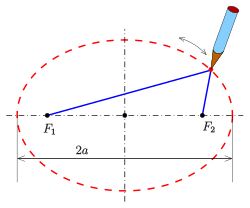
\includegraphics[width=0.5\textwidth]{Elliko-g.svg.png}
    \caption{ Called ``Garderner's Method" }
    \label{fig:}
\end{figure}

The notion is, there will be two points, it's the pivots. From here, the distance from the points to any random point of the ellipse is $r_1$ and $r_2$. The definition of ellipse is that the distance $r_1 + r_2$ is a constant. 

Let us say the distance $r_1 + r_2 = l$, which is a constant. 

The distance between the two pivot is $d$, thus, the string that we have, has a circumference (or the total length of the looped string) is $l + d$. 

\theo{  }{  }{ \emph{Ellipse} is the locus of all points that are positioned at distance $r_1$ and $r_2$ from two pivot points respectively. The rule is $r_1 + r_2$ is always  \emph{Constant}.    

    These pivot points may also be called ``Focus" in fancy language.
}

I know, calling this ``theorem" sucks. But who cares, we don't. 

Now this is all fine. But how can we find the equation, the specific function, that will give the plot of an ellipse, given $d$, $l$, and other necessary stuffs? 

It's not very hard though, we can do it. All we need to recap is that \emph{Cartesian Coordinates} is measured in $x,y$, hence the function my look like $f(x) = y$, and in case of \emph{Polar Coordinate}, measurements of positions is done in $r,\theta$, thus, a function may look like, $f( \theta) = r$.





Let one of the pivot be at $r= 0$, and the other one at $r= d$ along the horizontal axis. 
\begin{figure}[ht!]
    \centering
    \incfig{constellipsedraw}
    \caption{Drawing an Ellipse using strings, visualizing $r_1 + r_2 = l$ constant.}
    \label{fig:constellipsedraw}
\end{figure}

Here, we can find a few equations first,
\[ 
r_1 \cos \theta + r_2 \cos \alpha = d
\]
\[ 
r_1 \sin \theta = r_2 \sin \alpha
\]
\[ 
r_2 = l - r_1
\]
Now, using these equations, we do the following,
\begin{itemize}
    \item Eliminate $\alpha$ angle from the first equation. 
    \item Eliminate $r_2$ using $r_2 = l - r_1$ from the first. 
    \item Solve the first equation by keeping $r$ in one side.    
\end{itemize}
So, in quest of eliminating and solving the first equation, what we get is,
\[ 
    r_1 \cos \theta + \left( l-r_1 \right) \sqrt{1 - \left( \frac{r_1}{l- r_1} \right) ^2 \sin^2\theta} = d
\]  
It takes some amount of math to solve it, what we need is to find $r_1$ in one side of the equation. It isn't too hard though, what we end up with is,
\[ 
    r_1 = \frac{l^2 + d^2}{2 \left( l- d \cos \theta \right) }
\]
We can do a very quick sanity check, if the $d=0$, then what we essentially do is plot a circle (I drew a small picture in my notebook to visualize), now the reason is the two point is essentially a single point if distance between them is zero. So, the string ends up plotting circle. And it really does,\[ 
r_1 = \frac{l^2}{2 l } = \frac{l}{2}
\] Makes sense.

We can make things a little more tidy, let us factor off $l$ and say that $\frac{d}{l} = e$, 
hence,
\[ 
    r = \frac{l^2 \left(  1 + \frac{d^2}{l^2} \right) }{2l \left( 1-\frac{d}{l}\cos\theta  \right) }
\] 
And let us rename $\frac{l}{2 } = a$, hence,
\[
    \boxed{ r = \frac{a \left( e^2 + 1 \right) }{1 - e \cos \theta} }
\]
This is an \textbf{Equation of an Ellipse} in Polar Coordinates when one of the pivot or focus is our center/origin.

It's kind of nice, but then I tried to find some tricky way to isolate a method to find the tangent, but I learned I can't be Jaan Kalda so soon.

But I did find a way to manipulate an old realization of mine (that I probably have seen somewhere else too).


\newpage 
\section{ Projection of a Circle }
When I would go to the Mosque, I would look above where Ceiling Fan is spinning fast and making a clear cut circle. But the fans wouldn't look like circle if they weren't directly above the head, they would look like ``Ellipses".

Now, I naturally (or naively) assumed they are ellipses when looked from an oblique angle. And they are, but I don't know the proof yet. Well, we just proceed with our thought (it's correct though, but I say again I don't have the proof yet). 

I used this projection of 2D circle in an angle to make an idea what the tangent of an ellipse would look like.
\begin{figure}[ht]
    \centering
    \incfig{ellipses-are-oblique-circles}
    \caption{Ellipses are oblique Circles from the side view.}
    \label{fig:ellipses-are-oblique-circles}
\end{figure}
We have $\Gamma_1$ and $\Gamma_2$ circles. $\Gamma_2$ is as iff $\Gamma_1$ has been rotated and made at an angle with the horizontal, say angle is $\alpha$. If we project the $\Gamma_2$ on the circle $\Gamma_1$, we get an \emph{Ellipse}. 
This can be used to find the tangents of the ellipse.

\begin{figure}[ht]
    \centering
    \incfig{tangent-of-ellipse}
    \caption{Tangent of Ellipse}
    \label{fig:tangent-of-ellipse}
\end{figure}

Now, the circle is inclined with some angle. Say that the angle that the inclined circle makes with the horzontal plane as $\alpha$. If the circle $\Gamma_1$ has a tangent vector $\vec{v}$ and if it's inclined, then on the $\Gamma_2$ circle, the vertical component of the vector is going to look little smaller by some factor that depends on the angle the circle $\Gamma_{2}$ makes with the horizon. 

If the angle $\Gamma_2$ made with horizon was $0^{\circ}$, then the whole $\Gamma_2$ would look like parallel to surface and apparently $v_y' = 0$, the component of $\vec{v}$ along $\hat{y}$ would look zero. Draw some diagram, that will be clear.

This vector thing is drawn below.
\begin{figure}[ht!]
    \centering
    \incfig{the-vector-after-inclination}
    \caption{The vector after inclination}
    \label{fig:the-vector-after-inclination}
\end{figure}
From the diagram, the $\vec{v_y}$ starts to look like (apparently) $\vec{v_y} \sin \alpha$ after the inclining. And because of the direction of rotation, only the $y$ axis based components will seem to reduce in size. 

So the tangent of the Ellipse can be related with it's circle form (as we saw in the above figures),
\[ 
\vec{v} = v_x \hat{e_x} + v_y \hat{e_y}
\]
And the Ellipse has the counter part (after the tilting),
\[ 
\vec{v}' = v_x \hat{e_x} + v_y \sin \alpha \hat{ e_y}
\]

Now there is some caution to be maintained, looking at the figure, you can see that the vector $\vec{v}$ has it's tilted counterpart  to be exactly below it  along the $y$ axis. 

This makes sense. But the position of the vector here is necessary (as it is a tangent), and it has to be measured using the $x,y$ coordinates. Look the position of the tangent in circle and it's ellipse counterpart has same $x$ coordinate and the $y$ coordinate can be measured using simple trignonometry (because we know $\alpha$). 

Here, the position of the tangent has different values in Polar Coordinates. So be mindful about it. I have basically presented the idea, we can do various things with it. One thing that comes in my mind is finding area with it, or using it somehow to find the arc length or circumference of the ellipse (which turns out to be very hard). 

But there is a question that stil remains, \emph{What is the Eccentricity $e$ of the tilted circle $\Gamma_2$ which looks like ellipse in this case?}. Well, we can quickly do it.

Semi major axis is the half the longest line that joins two ends of the Ellipse. Semi minor is half of the shortest line that joins two points of ellipse.

If you draw an ellipse with the focus (or pivot) points in $x$ axis, the horizontal line across the ellipse is major axis (whose half is semi major axis) and the verticle one is semi minor. 

Now, in this case of tilted circle looking like ellipse, the semi major axis is $r$, which is the radius of the circle $\Gamma_1$. Assume that the tilted circle $\Gamma_2$ makes $\theta$ with the horizontal. 

The semi minor axis is $r \sin \theta$. Draw a diagram or refer to the one above. There is a relationship between semi minor and major axis. It can be found quickly from the equations that we have derived. But simply said, the relation is,
\[ 
\text{Semi Minor Axis} = \sqrt{1 - e^2}  \cdot \text{Semi Major Axis}
\]
Thus,
\[ 
r \sin \theta = \sqrt{1 - e^2}  r
\]
Solves, like this,
\[ 
e^2 = 1 - \sin ^2 \theta \to \boxed{  e = \cos \theta}
\]
Thus eccentricity is just $\cos \theta$. 

Now obviously there are some direct methods of finding tangents, I have some ninja techniques in my sleeve too. First of all, what is this tangent vector anyway?

So you have some implicit function, say, $\vec{r}\left( t \right) $, for example, this in expanded form,
\[ 
    \vec{r} \left( t \right)  = x\left( t \right)  \hat{e}_x +
    y\left( t \right) \hat{e}_y +
    z\left( t \right) \hat{e}_z
\]
Now, let's tweak $t$ by a little $\mathrm{d} t$ amount, what we have is,
\[ 
    \vec{r}\left( t + \mathrm{d} t \right)  - \vec{r}\left( t  \right) = \mathrm{d} \vec{r}
\] 
This small shift vector $\mathrm{d} \vec{r}$ is the direction where the tangent points, we can directly state that,
\[ 
\vec{\tau} = \frac{\mathrm{d} \vec{r}}{\mathrm{d} t}
\]
This is a nice thing. It directly yields a vector too. 

I tried this, and I got a result that was little intereting,
\[ 
    \hat{\tau} = \hat{\theta} - \frac{\hat{r}}{\sqrt{1 + e^2 - 2 e \cos \theta} }
\] I am not sure if this unit vector equation is correct or not.

















\section{ Finding Ellipse in Planet Orbits }
How about doing a very small recap? 

If you are familiar, feel free to skip some recap parts and start from the section \textbf{The Solution}


Gravity is the main force that acts on the bodies. We will assume our universe is full of mass. Thus, the first interaction we can think of them (that they do with each other, for example a star to a planet) is gravity. The two bodies $m_1$ and $m_2$ be located at $\vec{r_1}$ and $\vec{r_2}$, this means, 
\[ 
    \vec{F} = \frac{Gm_1m_2}{|\vec{r_2} - \vec{r_1}|^2} \frac{\vec{r_2} - \vec{r_1}}{| \vec{r_2} - \vec{r_1}|}
\]

If we can assume that the vector that joins the two mass is $\vec{r}$ and the dirction unit vector is $\vec{e}_r$, then, we can show this formula very shortly,
\[ 
\vec{F} = \frac{Gm_1m_2}{r^2} \vec{e}_r
\] 
Now, what will be the shape of the trajectory of a planet that is located at some distance from the star? 

From observation we can tell if the planet has some random initial speed, it will circulate around the star. Now, there must be a very well defined physics behind the system. 

We can use some mechanics to find out the \emph{shape} of the motion of planet around the star. There are some good conservation laws,
\begin{itemize}
    \item Energy Conservation law.
    \item Angular Momentum Conservation law.
\end{itemize}
Total Energy is shown by, 
\[ 
    E = \frac{1}{2} mv^2 + V(\vec{r})
\] 
Where $V(\vec{r})$ is the potential energy, which should be dependent on the position of the mass. $v$ is the velocity in any direction as usual. Angular momentum,
\[ 
L = mr^2 \omega
\] 
Here $\omega$ is the angular speed from the axis of rotation. 

We are ready to solve the problem of trajectory, shape of the path taken by a planet when it is moving around a star. 


\subsection{ The Problem }
\pk{ What is the shape of the trajectory when a planet of mass $m$ is moving around a star of mass $M $? Find the shape. }

I want to melt down this solution into some methods that we will follow by \emph{Finding the equation of motion using the Energy equation.}

\subsection{ Energy Method }
Let the total energy be written in this form. 
\[ 
    E = \frac{1}{2} m \dot{r}^2 + V(r)
\] Which only depends on one dimension $r$, and $ \dot{r} = \frac{\mathrm{d} r}{\mathrm{d} t}$ in short form, this is just the speed. This equation is perfect for the star-planet problem because here $r$ can be the distance between the two and $ \dot{r}$ is the \emph{radial speed}. If the rotation is of angular speed $\omega = \frac{\mathrm{d} \theta}{\mathrm{d} t} = \dot{\theta}$, hence, the tangential speed is $v_T = r\omega = r \dot{\theta}$.


The problem can be handled by plugging everything in place, the total kinetic energy is the sum of the tangential and radial speed, the potential energy can be found later. 

But now, if we take a derivative $ \frac{\mathrm{d} E}{\mathrm{d} t}$, what we find is,
\[ 
\frac{\mathrm{d} E}{\mathrm{d} t} =
\frac{1}{2}m \left( \frac{\mathrm{d} }{\mathrm{d} r} \dot{r}^2 \right) 
+ 
\frac{\mathrm{d} }{\mathrm{d} t} \left( V(r) \right) 
\]
By the chain rule of differentiation, we know,
\[ 
    \frac{\mathrm{d} f(x)}{\mathrm{d} t} = \frac{\mathrm{d} f}{\mathrm{d} x} \frac{\mathrm{d} x}{\mathrm{d} t}
\]
Hence,
\[ 
\frac{\mathrm{d} E}{\mathrm{d} t}=
\frac{1}{2} m 
\left( 2 \dot{ r} \ddot{ r } \right) + 
\frac{\mathrm{d} V(r)}{\mathrm{d} r} \frac{\mathrm{d} r}{\mathrm{d} t}
=
m \ddot{ r } + \frac{\mathrm{d} V(r)}{\mathrm{d} r}
\]
We can factor out $ \dot{r}$, and because the energy is constant always, $ \frac{\mathrm{d} E}{\mathrm{d} t} = 0$, hence,
\[ 
    m \ddot{ r } = - \frac{\mathrm{d} V(r)}{\mathrm{d} r}
\]
This is a result which we could find in the other way. Notice that $\ddot{ r }= \frac{\mathrm{d} ^2}{\mathrm{d} t^2}r= a$ which is acceleration. Hence this above equation is just newton's second law from the energy conservation rule. We will use this extensively to find the total path of motion of planet.

So let us summarize, 
\theo{   }{ Energy Rule }{ If the total energy can be written as, 
\[ 
    E = \frac{1}{2} m \dot{r}^2 + \Pi(r)
\]
then,
\[ 
    m \ddot{r} = - \frac{\mathrm{d} \Pi(r)}{\mathrm{d} r}
\] Please note, there must be a single dimension of choice only. 
}
\subsection{ Finding the Total Energy Equation }
We are here with the energy,
\[ 
    E = \frac{1}{2} m v_T ^2 + \frac{1}{2} m v_r ^2 + V(r)
\]
This is, 
\[ 
    E = \frac{1}{2} m \left( \dot{r}^2 + r \dot{\theta}^2 \right) + V(r)
\]
Here is a problem, $ \dot{\theta}$ is another dimension (in polar coordinate $r,\theta$ are two separate dimension), but this isn't a big problem as we can use the Angular Momentum,
\[ 
L = mr^2 \dot{\theta} \to \theta = \frac{L}{mr^2}
\]
Putting this in place,
\[ 
    E = \frac{1}{2} m \dot{r}^2 + \frac{L^2}{2mr^2} + V(r)
\]
Now check that this problem is just one dimensional, because it only depends on $r$.

\subsection{ The Solution }
Total energy is here,

\[ 
    E = \frac{1}{2} m \dot{r}^2 + \frac{L^2}{2mr^2} + V(r)
\]

Now, the $ \dot{r}$ term is for the kinetic energy, the rest must be for potential energy, the dimension we depend on is $r$, hence,
\[ 
    E = \frac{1}{2} m \dot{r} ^2 + \Pi(r)  = \frac{1}{2} m \dot{r}^2 + \frac{L^2}{2mr^2} + V(r)
\]
Thus, the effective potential energy in this case, 
\[ 
    \Pi(r) = \frac{L^2}{2mr^2} + V(r)
\]

Hence, using the energy rule we found,
\[ 
    m \ddot{ r } = \frac{\mathrm{d} \Pi}{\mathrm{d} r} = \frac{L^2}{mr^3} - F(r)
\]
But the problem is, we have now found, \[ 
\frac{\mathrm{d} ^2 r}{\mathrm{d} t^2}
\]but to find the shape, we have to find, 
\[ 
\frac{\mathrm{d} ^2r}{\mathrm{d} \theta^2}
\] We have to change the variable.

No problem, we can use chain rule, 
\[ 
\frac{\mathrm{d} r}{\mathrm{d} t} = \frac{\mathrm{d} r}{\mathrm{d} \theta} \frac{\mathrm{d} \theta}{\mathrm{d} t} = \dot{\theta } \frac{\mathrm{d} r}{\mathrm{d} \theta} 
\]
And the math is easier to do using $u$ instead of $r$, if $r = \frac{1}{u}$. Let us solve for $\dot{ \theta }$ in terms of $u$, 
\[ 
\dot{\theta} = \frac{L}{mr^2} = \frac{Lu^2}{m}
\]
\[ 
\frac{\mathrm{d} r}{\mathrm{d} t} =
\left( L \frac{u^2}{m} \right) \frac{\mathrm{d} r}{\mathrm{d} \theta}
=
\frac{\mathrm{d} }{\mathrm{d} \theta} \left( \frac{1}{u} \right) = \left( \frac{Lu^2}{m} \right) \left( - \frac{1}{u^2} \frac{\mathrm{d} u}{\mathrm{d} \theta} \right) 
\]
This finally yields,
\[ 
\frac{\mathrm{d} r}{\mathrm{d} \theta} = 
- \frac{L}{m} \frac{\mathrm{d} u}{\mathrm{d} \theta}
\] 
Hence, we can easily find,
\[ 
\frac{\mathrm{d} ^2 r}{\mathrm{d} t^2} = - \frac{L}{m} \frac{\mathrm{d} }{\mathrm{d} t}
\left( \frac{\mathrm{d} u}{\mathrm{d} \theta} \right) =
- \frac{L}{m} \left( \frac{\mathrm{d} 
\frac{\mathrm{d} u}{\mathrm{d} \theta}
}{\mathrm{d} \theta} \cdot  \frac{\mathrm{d} \theta}{\mathrm{d} t} \right) = - \frac{L}{m} \frac{\mathrm{d} ^2 u}{\mathrm{d} \theta^2 } \dot{\theta}
=
- \frac{L}{m} \left( \frac{L}{mr^2} \right) \frac{\mathrm{d} ^2 u}{\mathrm{d} \theta^2}
\] 
So,
\[ 
\frac{\mathrm{d} ^2 r}{\mathrm{d} t^2} =
- \left( \frac{L^2}{m^2 r^2} \right) \frac{\mathrm{d} ^2 u}{\mathrm{d} \theta ^2}
\]
Using this in the equation of motion, (the equation that finds $\ddot{ r }$ ), 
\[ 
    - \frac{L^2}{m r^2} \frac{\mathrm{d}^2 u}{\mathrm{d} \theta^2} = \frac{L^2}{m}u^3 -F(u)
\]
\[ 
    \frac{\mathrm{d} ^2 u}{\mathrm{d} \theta^2} = \frac{m}{L^2 u^2} F(u) - u
\]

So, the final differential Equation,
\[ 
\boxed{ 
    \frac{\mathrm{d} ^2 u}{\mathrm{d} \theta^2} + u - \frac{m}{L^2u^2}F(u) = 0
}
\]  
This can also be seen as,
\[
    \boxed{ \frac{\mathrm{d} ^2}{\mathrm{d} \theta^2} \left(\frac{1}{r} \right) + \frac{1}{r} - \frac{mr^2}{L^2 } F\left( r \right) =0}
\]


\subsection{ The Differntial Equation }
What is the use of this differential equation? Using this, we can solve for $r(\theta)$. This is the polar equation that will trace the path of the particle in gravitational force. Now, in case of Newtonian Gravity, the force $F(r)$ is, 
\[ 
    F (r) = -\frac{Gm_1m_2}{r^2} \to F(u) = - \frac{Gm_1m_2}{1} u^2 = - G m_1 m_2 u^2
\] 
The equation is, then,
\[ 
\frac{\mathrm{d} ^2 u}{\mathrm{d} \theta^2} + u + \frac{m}{L^2 u^2} G m_1 m_2 u^2 = 0
\]
Solving,
\[ 
\frac{\mathrm{d} ^2 u}{\mathrm{d} \theta ^2} + u + k = 0
\]
Here $k$ is used to replace some constant terms, we don't at all need to deal with them.
We need to \textbf{solve} this differential equation using basic ninja techniques, the reason is because the direct and general solution is hard to find and uses difficult techniques, we can solve it using some basic general physics knowledge.

For the types of differential equations we are seeing here, they can be solved by assuming,
\[ 
u = u_g + u_p
\]
Here $u_g$ is the ``Homogenous" solution. Why? It's just the method. $u_p$ is the particular solution. Using this, 
\[ 
\frac{\mathrm{d} ^2 u_g}{\mathrm{d} \theta^2} + u_g = 0
\]
\[ 
u_p + k = 0 \to u_p = -k
\]
Solution to $u_g$ is,
\[ 
    u_g = A \cos(\theta + \phi) 
\]
This means the solution is,
\[ 
    u = A \cos \left( \theta + \phi \right) - k
\]
This solution is a standard solution to the differential equation, $\ddot{ r }+ r = 0$
And using $r$ instead of $u$,
\[ 
    r = \frac{1}{A \cos \left( \theta + \phi \right) - k}       
\]
Get rid of random constants and simplify it, I will take factor of $-k$, set $-\frac{A}{k} = e$, and by putting $\alpha$ as $\frac{1}{-k}$, setting initial $\theta = 0$ hence, $\cos\phi  \to \phi = 0$ this shows,
\[ 
    r = \frac{1}{-k \left( 1 + e \cos \theta \right) } 
\]
\[ 
r = \frac{\alpha}{1 + e \cos \theta}
\]
Let at $\theta = 0$, $r=r_0$, this is,
\[ 
r = r_0 = \frac{\alpha}{1 + e}
\]
If $\alpha = r_0 \left( 1 + e \right) $, then, 
\[ 
    r_0 = \frac{r_0 \left( 1 + e \right) }{1 + e} = r_0
\]
This solves, the equation so that, 
\[ 
    \boxed{ r = \frac{r_0 \left( 1 + e \right) }{1 + e \cos \theta}}
\]
This $r$ is a solution to the equation. What if $e=0$? 
\[ 
r = r_0 
\] That means for all  $\theta$, the distance is always going to be $r_0$, that means circle.It is very interesting to notice. And what if we plot our newly found equation $r(\theta)$ in a graph paper? Let us plot the current mathematica code for some random values.

\begin{verbatim}
r0 = 10
e = 0.7 
PolarPlot[(r0 * (1 + e)/(1 + e*Cos[\[Theta]])), {\[Theta], 0, 2*Pi}] 
\end{verbatim}

\begin{figure}[ht!]
    \centering
    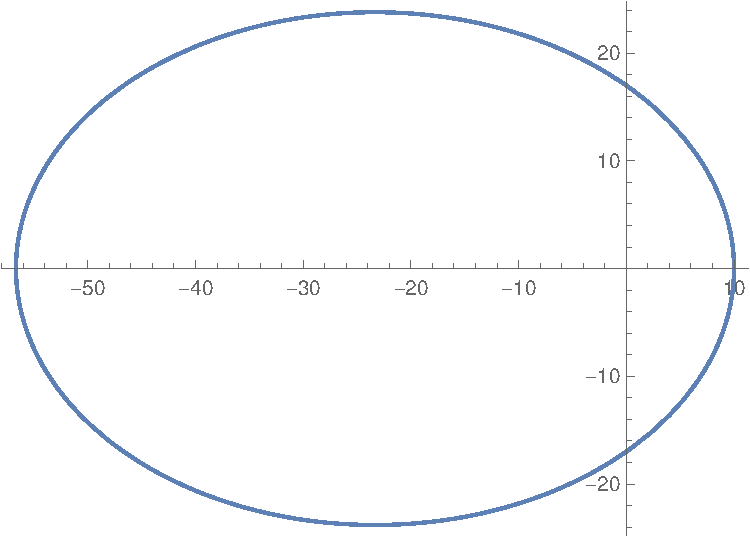
\includegraphics[width=0.4\textwidth]{aellipse.pdf}
    \caption{Plotting the function we found with $r_0=10$ and $e = 0.7$}
    \label{fig:}
\end{figure}

Which looks like an ellipse and it is an ellipse. Looking closely, the center is the position of the star, relative to it we measure $r$, and the minimum distance is $r=10$ which is $r_0$. Maximum distance from center is at $\theta = 180^{\circ}$, which is, 
\[ 
r = r_0 \frac{1+ e}{1 - e}
\]
Let us use another ninja technique, say maximum distance from the focus is, $a + ea$ or $a \left( 1 +e \right) $ and lowest distance is $a - ea$ or $a \left( 1 -e \right) $, then, 
\[ 
    r_0 = a \left( 1 -e \right) 
\] 
And maximum,
\[ 
    r_{ max } = a\left( 1 -e \right) \frac{1+e}{1-e} = a\left( 1 + e \right) 
\] That is valid. 
This $a$ has a special name, which is semi major axis. Why? Add  the minium and maximum distance,
\[ 
    D = a(1+e) + a(1-e) = 2a
\]Here, $D$ is the addition of minimum and maximum distance, which is just the horizonatal line that joins the two extreme points of the ellipse, and this line that joins the two ends is the major axis. Half of it is $a$, thus $a$ is called  \emph{Semi Major Axis}.


Now a small add to the story, note  that this differential equation can also be used when there is more than gravitational force, because all we need is a general $F(r)$ equation that can be anything. Hence, we can also find General Relativistic Gravity Paths, because in General Relativity, the Equivalent force (which is not technically force though) can be written as,
\[ 
    F(r) = k_1 \frac{1}{r^2} + k_2 \frac{1}{r^3} = k_1 u^2 + k_2 u^3
\]
The shape of this sort of path is more different than what we found now.
\\
\solu{ Hence the Path that a planet would trace around a Star is an \emph{Ellipse}  

The path is give in the polar coordinates as a funciton $r\left( \theta \right) $, which is, by $r_0$ being the minimum distance to center,
\[ 
r\theta = r_0 \frac{1 + e}{1 + e \cos \theta} 
\]
In terms of semi major axis $a$, that is more convinient in Astronomy,
\[ 
    r\left( \theta \right)  = a \frac{1 - e^2}{1 + e \cos \theta}
\]
The equation also precludes the center of the reference is one of the focus of the ellipse.
}

\subsection{ Few more thoughts on it }  
Now because this ellipse equation is a result, it makes me think why it has to be?

Well someone else has answered this question before us, it's Euler and Lagrange and other smart people.

The reason why the solution is an Ellipse is because there is some property in ellipse that else don't have.

I mean, this orbit could have been like a squre, or a rectangle form, or it could be stricly a circle whatever the cause be. But it's elliptical. And not just elliptical to be honest, it can be any conic section because of the form $r = \frac{1}{\left( 1+ e \cos \theta \right) ^2}$. 

Now from Euler Lagrangian Equation, and the Idea of Analytical Mechanics, there is a quantity called the action,
\[ 
    A = \int_{ }^{} L[t, \dot{r}, \ddot{ r }] \mathrm{d} t  
\]
This quantity $A$ has to be Stationary (or minimum or maximum) for it to be appearing in nature. Hence, we need to know the special equation $L$ that will make $A $ stationary with respect to others possible values.

$L$ directly depends on the equation of the path, it's shape. For every point along the trajectory, $L$ has some value. And it is such that, $A$ always has stationary value. 

For an integral like A (as we wrote) to be stationary, the function $L$ has to satisfy this equations, 

\[ 
\frac{\mathrm{d} }{\mathrm{d} t} \frac{\partial L}{\partial \dot{r}} = \frac{\partial L}{\partial r}
\]

For mechanics, we know the value of $L$, which is,
\[ 
L = T - V
\]
Probably that's how we solve this problem.

We can try calculating the value of $A$ for anyother Unorthodox path, like a square instead of ellipse, it would probably have a non stationary value for $A$. 


\section{ A very cool problem }
We almost always would ignore curvature of Earth while solving any projectile problem. The problem be like,

\pk{ We through a mass $m$ from this and this position, where will it land? \emph{Ignore Curvature of Earth}, and the angle of throwing the mass is $\theta$.  }

Now, it's not hard to use the equation of Parabolic Trajectory and solve it (I recall writing a handout on this). But what if we don't ignore curvature of Earth?

\pk{ Solve the problem of mass falling as before, but \emph{Don't Neglect Curvature of Earth}.  }

It's, to be honest, not too hard to solve either.

Because, the central feature is, in case of such non approximating cases, the projectile is just elliptical in nature. 

\begin{figure}[ht!]
    \centering
    \incfig{projectile-in-reality-is-just-an-ellipse.}
    \caption{Projectile in reality is just an ellipse.}
    \label{fig:projectile-in-reality-is-just-an-ellipse.}
\end{figure}


The focus of the ellipse is just the center of earth, and solving this for a spherical earth is very easy because $r=r$ in the landing and falling case. So, even though avoiding an approximation, we still don't have a very tough situation (which is kinda rare).

Thanks to Arnab vai for sharing this idea. 


\section{ The problem of Illumination }
\pk{ Given a bounded region, which is made by Walls. These wall's are reflective. Given at any point inside the bounded region Walls, there is a point like light bulb, from which light radiates, find all the points in the region where light doesn't reach, and it is dark. }

Well, simply said, if the region is square, then if any light source is inside, all points in the region is going to be illuminated. Now for random boundary, we need the dark points. 

Ellipses has this capability. That there is a focus. And if you light a bulb just at the focus point, all the light will eventually end up in the other focus. 

Well, you can make a billiard board, and shape it in ellipse. Now, if you cut a hole in one of the focus, then hitting the ball from the other focus will always and always put that ball in hole.

To me it was a fascinating thing, so should to you (unless you are Terry Tao and have derived it yourself at the age of three :yaw: ) 

Check "Playing Billiard with Maths" by Numberphile in Youtube. 

Now, for the illumination problem, it also has a Numberphile video. I won't give the links, I don't want to open the browser now, but you can find it using the "illumination problem" keyword. 

Roger Penrose (boss music begins) solved it. The problem is tackled using ellipses. If you accompany yourself with the idea, that light emitted from Focus will end up in the other focus, you can have a clearer understanding of the Numberphile video I mentioned.
















\newpage

\section{ Area of Ellipse }
Keplar's Laws has some dependency on the area of ellipses. This motivates us to find the area of it.

Now, we can trick the solution and find the area very quickly. But in my case, just after I derived the polar coordinate equation (using the string method), I tried deriving the area from that using brute force. 

\begin{figure}[ht!]
    \centering
    \incfig{area-of-ellipse-in-polar-coordinate-form}
    \caption{Area of ellipse in polar coordinate form}
    \label{fig:area-of-ellipse-in-polar-coordinate-form}
\end{figure}

The small triangle has area $\mathrm{d} A$ which is,
\[ 
    \mathrm{d} A = \frac{1}{2} r \left( r \mathrm{d} \theta \right) 
\]
The complete area with the full integral,
\[ 
A=\int_{0}^{2 \pi} \frac{1}{2} r^2 \mathrm{d} \theta 
\]
Now, we have $r$, so, ignoring all constant terms, we have to solve for an integral,
\[ 
    I = \int_{0 }^{2\pi} \left( \frac{1}{1 + e \cos \theta} \right) ^2 \mathrm{d} \theta 
\]
And here it comes, the integral that took me a very good amount of time to be unable to solve eventually. 

It's a tough integral. I thought using $\beta$ functions or $\Gamma$ function might work, but no they don't.

I thought that expanding a Taylor Series had potential but I didn't try it. I had to look quite a while until someone posted a nicely written solution in Physics Stack Exchange. 

Here is the solution, from someone in Physics Stack Exachange.

Start by forgetting unncessary stuffs,
\[ 
    I = \int_{0}^{\theta} \frac{\mathrm{d} \theta}{(1 + e \cos \theta)^2} 
\]
Now, change the variable with the most epic substitution ever (that I have no idea why),
\[ 
\tan \frac{\theta}{2} = z \to \cos \theta = \frac{1 - z^2}{1 + z^2}
\]
\[ 
\mathrm{d} \theta = \frac{z \mathrm{d} z}{1 + z^2}
\]
Now the integral is,
\[ 
    I = \int_{ }^{} \frac{\left( 1  + z^2 \right) \mathrm{d} z}{\left(z^2 + 
    \frac{1 + e}{1-e} \right)^2
    }  
\]
Then, making the thing a little more easy by,
\[ 
\frac{1+e}{1-e} = k
\]
by using ``Ostrogradsky's" method, this integral is now,
\[ 
I = \left[
    \frac{1-k}{2k} \cdot \frac{\tan \frac{\theta}{2}}{\tan ^2 \frac{\theta}{2} + k} +
    \left( \frac{1+k}{2k} \right) + \frac{1}{\sqrt{k} }\cdot \arctan \left(  \frac{\tan \frac{\theta}{2}}{\sqrt{k} }  \right)  
\right]_{ 0 }^{ \theta }
\]
Using appropriate constants that we were ignoring so far, 
\[ 
    \boxed{  A = \pi a b}
\]
Where $a$ is Semi Major Axis and $b$ is Semi Minor Axis.

I don't know the ``Ostrogradsky's" method, I think that a good manipulation of the Beta and Gamma function might be useful to solve this integral. What is Beta and Gamma function? They are just some fancy method I found in Flammable Maths youtube channel in the video where he solves the Pendulum equation of motion exactly,
\[ 
\ddot{ \phi } + \omega^2 \sin \phi = 0
\]
There is use of this special equation which is a form of beta function,
\[ 
    \beta\left( m,n \right) = 2 \int_{0}^{\frac{\pi}{2}} \sin ^{2m -1} \theta \cdot  \cos ^{2n-1} \theta \mathrm{d} \theta 
\]
And the $\beta$ function itself is, in relation to $\Gamma$ function.
\[ 
    \beta(m,n) = \frac{\Gamma\left( n \right) \Gamma\left( m \right) }{\Gamma\left( m+n \right) }
\]
And $\Gamma$ function is,
\[ 
    \Gamma(n) = \int_{0}^{\infty} x^{n-1} e^{-x} \mathrm{d} x 
\] 
Another form of it is,
\[ 
    \Gamma(n) = \lim_{m \to \infty} \frac{1\cdot 2\cdot 3\cdot \ldots m}{n \left( n+1 \right) \left( n+2 \right) \ldots \left( n+m \right) } m^{n}
\]
The thing is, these can be manipulated in various ways that give solutions to tough integrals. 
Let me term a problem and show it's solution,
\pk{ 
Solve the integral,
\[ 
I = \int_{0}^{1}  \frac{\mathrm{d}  x}{\sqrt{1 - x^{n}} } 
\]
}   
\solu{ To evaluate, use,
\[ 
x^{n} = \sin^2\theta
\], that yields,
\[ 
    \mathrm{d} x = \frac{2}{n} \left( \sin \theta \right) ^{\left( 2-n \right) / n } \cos \theta \mathrm{d}  \theta
\]
 Then putting this in the place of integral,
 \[ 
     I = \frac{2}{n} \int_{0}^{1} \left( \sin \theta \right) ^{\left( 2 - n \right) / n} \mathrm{d} \theta 
 \]
 Now, we know this can be represented as a $\beta$ function, because,
 \[ 
     \beta \left( m,n \right) = 2 \int_{ 0 }^{\frac{\pi}{2}} \sin ^{2m-1} \theta \cos ^{2n-1}\theta \mathrm{d}  \theta
 \] 
 Using appropriate $m,n$ values, we can use this to solve the required integral, which is,
 \[ 
     I = \frac{2 \Gamma\left( \frac{1}{2} \right) \Gamma\left( \frac{1}{n} \right) }{n \cdot  2 \Gamma\left( \frac{1}{n} + \frac{1}{2} \right) }
 \] 
 Using that factorial or numerical definition, it's not hard to find out the solution numerically given the value of $n$.
}

























\end{document}
